\documentclass[12pt]{article}

\usepackage[T1]{fontenc}
\usepackage{inter} 
\renewcommand*\familydefault{\sfdefault}
\usepackage{geometry}
\setlength{\textwidth}{6.5in}
\geometry{
    a4paper,
    top=1.8cm,
    bottom=1in,
    left=1cm,
    right=1cm
}

\setcounter{secnumdepth}{0} % remove section numbering
\pdfgentounicode=1 % make ATS friendly

\usepackage{enumitem}
\setlist[itemize]{
    itemsep=1pt,
    left=0.3em
}
\setlist[description]{itemsep=1pt}
\setlist[enumerate]{align=left}
\usepackage[dvipsnames]{xcolor}
\usepackage{color,graphicx}
\definecolor{blue}{RGB}{0,102,204}
\definecolor{iconblue}{RGB}{30,109,220}
\colorlet{icnclr}{gray}
\usepackage{titlesec}
\titlespacing{\subsection}{1pt}{1pt}{1pt}
\titlespacing{\subsubsection}{1pt}{1pt}{1pt}
\titleformat{\section}{\color{blue}\large\fontseries{black}\selectfont\uppercase}{}{}{\ruleafter}[\global\RemVStrue]
\titleformat{\subsection}{\fontseries{bold}\selectfont}{}{}{\rvs}
\titleformat{\subsubsection}{\color{gray}\fontseries{bold}\selectfont}{}{}{}

\usepackage{xhfill} 
\newcommand\ruleafter[1]{#1~\xrfill[.5ex]{1pt}[blue]} % add rule after title in .5 x-height 

\newif\ifRemVS % remove vspace between \section & \subsection
\newcommand{\rvs}{
    \ifRemVS
        \vspace{-1ex}
    \fi
    \global\RemVSfalse
}

\usepackage{fontawesome5}

\usepackage[bookmarks=false]{hyperref} % [imp!]
\hypersetup{ 
    colorlinks=true,
    urlcolor=iconblue,
    pdftitle={My Resume},
}

\usepackage[page]{totalcount}
\usepackage{fancyhdr}
\pagestyle{fancy}
\renewcommand{\headrulewidth}{0pt}	
\fancyhf{}							

\usepackage{amsmath}
\usepackage{amsfonts}

\begin{document}

%== HEADER ==%

\begin{flushleft}
    {\fontsize{30}{30}\selectfont Revathy Venugopal} \\ \bigskip
    
    {\color{icnclr}\faMapMarker} {Lyon, France} \\ \bigskip
    {\color{icnclr}\faEnvelope[regular]} \href{mailto:revathyvenugopal162@gmail.com}{revathyvenugopal162@gmail.com} \\ \bigskip
    {\color{icnclr}\faIcon{mobile-alt}} \href{tel:+33769359272}{+33 769359272} \\ \bigskip
    % You can also put your LinkedIn or website address
    {\color{icnclr}\faLinkedinIn} \href{https://www.linkedin.com/in/revathy-venugopal-3310b5147/}{Revathy Venugopal}\\ \bigskip
    {\color{icnclr}\faGithub} \href{https://github.com/Revathyvenugopal162/}{Revathy Venugopal}
\end{flushleft}
\noindent
\hfill
\raisebox{0pt}[0pt][0pt]{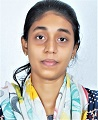
\includegraphics[width=0.3\textwidth]{../assets/revathy.jpg}}
%==============
%==============
%==============
\noindent
Innovative and passionate \textbf{software developer}, seeking to leverage extensive background in Software development.
Proficient in Python programming, I have successfully developed and maintained multiple scalable and efficient software applications.
Demonstrated strong problem-solving skills by implementing optimised algorithms and data structures in Python, significantly improving system performance.
%==============
%==============
\section{Experience}
%==============
%==============
\subsection{R and D Engineer \hfill \normalfont May 2022-- Present} \\ \smallskip
\subsubsection{Ansys, France} \\ \smallskip
% Start all items with action verbs
\begin{itemize}
    \item[\textbullet] Python Development: Build efficient applications using Python.
    \item[\textbullet] Sphinx Documentation: Write and manage project documentation with Sphinx.
    \item[\textbullet] Best Practices in Software Development: clean code and thorough testing.
    \item[\textbullet] GitHub: Use GitHub for version control and collaboration.
    \item[\textbullet] CI/CD: Implement CI/CD pipelines for automated testing and deployment.
    \item[\textbullet] RAG-Based LLM Development, AI/ML: Develop RAG-based LLM using AI/ML.
\end{itemize}

\subsection{Machine Learning And Robotics Intern \hfill \normalfont September 2021-- April 2022} \\ \smallskip
\subsubsection{SITIA Robotique, Nantes} \\ \smallskip
% Start all items with action verbs
\begin{itemize}
    \item[\textbullet] Python-Based Software, Obstacle Detection, TensorFlow, OpenCV: Developed software and algorithms for robot vision and obstacle avoidance.
\end{itemize}

%==============
%==============
\section{Professional Qualification}
%==============
%==============
\subsection{Master of Science in Embedded Systems \hfill \normalfont 2020 - 2022} \\ \smallskip
\subsubsection{ESIGELEC, Rouen, France} \\ \smallskip
\begin{itemize}
    \item[\textbullet]Embedded systems, software development, machine learning, robotics, computer vision
\end{itemize}

\subsection{Master of Engineering in Embedded Systems \hfill \normalfont 2020 - 2022} \\ \smallskip
\subsubsection{MAHE, Manipal, India} \\ \smallskip
\begin{itemize}
    \item[\textbullet] Automotive embedded systems, software development, machine learning, robotics, computer vision, IOT, embedded C, Real-time operating systems
\end{itemize}

\subsection{Bachelor of Technology in Electrical and Electronics Engineering \hfill \normalfont 2014 - 2018} \\ \smallskip
\subsubsection{College of Engineering, Munnar, India} \\ \smallskip
\begin{itemize}
    \item[\textbullet] Electrical and electronics engineering, power systems, electrical machines, control systems, power electronics
\end{itemize}

%==============
%==============
\section{Skills}
\subsection{Technical} \smallskip
\begingroup
\setlength{\tabcolsep}{1pt}
\begin{tabular}{p{0.35\textwidth} p{0.35\textwidth} p{0.35\textwidth}}
    \textbullet Python & \textbullet JavaScript & \textbullet C \\
    \textbullet CSS & \textbullet HTML & \textbullet Docker \\
    \textbullet Tensorflow  & \textbullet OpenCV & \textbullet PyTorch \\
    \textbullet LaTeX 
\end{tabular} \smallskip

\subsection{Soft Skills} \smallskip
\begingroup
\setlength{\tabcolsep}{0pt}
\begin{tabular}{p{0.35\textwidth} p{0.35\textwidth} p{0.35\textwidth}}
    \textbullet Problem-solving & \textbullet Teamwork & \textbullet Communication \\
    \textbullet Adaptability & \textbullet Time management & \textbullet Leadership \\
    \textbullet Critical thinking & \textbullet Creativity & \textbullet Emotional intelligence \\
    \textbullet Conflict resolution & \textbullet Decision-making & \textbullet Stress management \\
\end{tabular} \smallskip

\subsection{Tools} \smallskip
\begingroup
\setlength{\tabcolsep}{0pt}
\begin{tabular}{p{0.35\textwidth} p{0.35\textwidth} p{0.35\textwidth}}
    \textbullet GitHub & \textbullet Git & \textbullet Bitbucket \\
    \textbullet Jupyter notebook & \textbullet Sphinx & \textbullet CI/CD \\
\end{tabular} \smallskip

\subsection{Languages} \smallskip
\begingroup
\setlength{\tabcolsep}{0pt}
\begin{tabular}{p{0.35\textwidth} p{0.35\textwidth} p{0.35\textwidth}}
    \textbullet English & \textbullet French 
\end{tabular} \smallskip
\endgroup

%==============
%==============
\section{Additional Education}
\subsection{Using Python to Access Web Data \hfill \normalfont 2021} \\ \smallskip
\subsubsection{Coursera}
\begin{itemize}
    \item[\textbullet]Python, web data, web scraping, web services, XML, JSON
\end{itemize}
\subsection{Introduction to Programming Using Python \hfill \normalfont 2020} \\ \smallskip
\subsubsection{Coursera}
\begin{itemize}
    \item[\textbullet] Python, programming, data structures, algorithms
\end{itemize}
\subsection{Python Data Structures \hfill \normalfont 2020} \\ \smallskip
\subsubsection{Coursera}
\begin{itemize}
    \item[\textbullet] Python, data structures, algorithms, programming
\end{itemize}
%==============
%==============
%==============
\end{document}
